\section{Propagation across a thin cylinder}\label{sec:cylinder}

The energy of Proposition \ref{prop:fibre} controls the wave on the circle $|\tau|=2a$ for
$1\le T\le2$, and is controlled by the data on $|\tau|=4a$ at $T=0$. To compare the two sets we
first carry the energy out to $|\tau|=1$, where a fixed neighbourhood connects the two time
intervals, and then carry it back towards the inner wall. Each passage costs one logarithm, as
Figure \ref{fig:cylinder} illustrates. The radial harmonic functions used for comparison are the
probabilities that planar Brownian motion leaves an annulus through one circle or the other
\cite[Theorem 3.18]{MP10}; the maximum principle keeps this comparison in the presence of a
potential.

\begin{figure}[t]
\centering
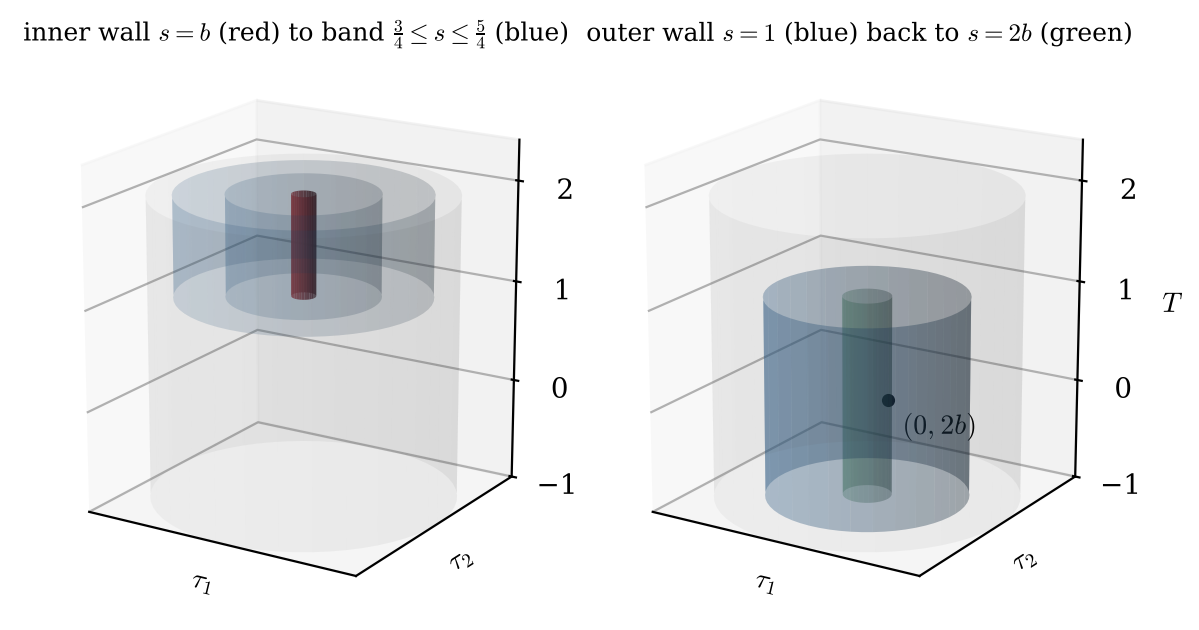
\includegraphics[width=0.95\textwidth]{figures/fig_cylinder.png}
\caption{The two comparisons in the $(T,s)$ half-plane, $s=|\tau|$, drawn schematically. Left: the
mass of the circular mean on the inner wall $s=b$ for $1\le T\le2$ bounds the mass in the band
$3/4\le s\le5/4$ from below, at the cost $1/\log(3/b)$. Right: a mean-value inequality on a fixed
annulus gives a lower bound on the whole outer wall $s=1$, and the comparison solution
$\cos(\pi T/2)u(s)$ carries it back to $s=2b$ at the cost $\log 2/\log(1/b)$. In the wave estimate
$b=2Kh$, the inner wall controls the wave on $1\le T\le2$, and the dot at $(0,2b)$ is controlled by
the initial data.}
\label{fig:cylinder}
\end{figure}

\begin{lemma}[\cite{OAI26}]\label{lem:cylinder}
Let $0<b<1/4$ and $D=\log(3/b)$. Suppose a continuous potential $V:[b,3]\to[0,\infty)$ satisfies
\begin{equation}\label{eq:Vint}
\int_b^3s\log(s/b)\,V(s)\,ds\le M,\qquad\sup_{1/2\le s\le3/2}V(s)\le M .
\end{equation}
Let $E\ge0$ be smooth on $\R_T\times\{\tau\in\R^2:b\le|\tau|\le3\}$ with
$\Delta_{T,\tau}E\le V(|\tau|)E$ in the interior. Its circular mean
\[
H(T,s)=\frac1{2\pi}\int_0^{2\pi}E\bigl(T,s(\cos\theta,\sin\theta)\bigr)\,d\theta
\]
satisfies, for $b\le r\le1$,
\begin{equation}\label{eq:cylinder}
H(0,r)\ge c(M)\,\frac{\log(r/b)}{D^2}\int_1^2H(T,b)\,dT .
\end{equation}
In particular the factor at $r=2b$ is a constant multiple of $D^{-2}$.
\end{lemma}

\begin{proof}
Averaging over rotations preserves the differential inequality, so $H(T,|\tau|)$ is again a
supersolution: $(-\Delta_{T,\tau}+V)H\ge0$. All maximum principles below are the weak maximum
principle for operators $\Delta-c$ with bounded $c\ge0$ \cite[Corollary 3.2]{GT01}.

\emph{Radial comparison functions.} For $S\in\{1,3\}$ and a fixed $\kappa>0$ consider
\[
u''+s^{-1}u'=(V+\kappa^2)u\qquad(b<s<S),
\]
with endpoint values $0,1$ in either order. We claim that $u$ is at least a constant $c(M,\kappa)$
times the function affine in $\log s$ with the same endpoint values. The substitution
$x=\log(s/b)$ gives $u''+s^{-1}u'=s^{-2}u_{xx}$, so the equation becomes $u_{xx}=P(x)u$ on $[0,A]$
with $A=\log(S/b)$ and $P(x)=s^2(V(s)+\kappa^2)\ge0$. Let $\psi$ solve it with $\psi(0)=0$,
$\psi'(0)=1$. Then $\psi''=P\psi\ge0$ while $\psi\ge0$, so $\psi'\ge1$ and $\psi(x)\ge x$. Integrating
twice, $\psi(x)=x+\int_0^x(x-z)P(z)\psi(z)\,dz$, that is,
\[
\frac{\psi(x)}x=1+\int_0^x\frac{z(x-z)}{x}\,P(z)\,\frac{\psi(z)}z\,dz .
\]
Since $z(x-z)/x\le\min(z,A-z)$, Gronwall's inequality gives
$\psi(A)/A\le\exp\bigl(\int_0^A\min(z,A-z)P(z)\,dz\bigr)$. In this integral, $dz=ds/s$ and
$\min(z,A-z)\le\log(s/b)$, so the contribution of $V$ is at most
$\int_b^3s\log(s/b)V(s)\,ds\le M$; with $t=A-z$, $s=Se^{-t}$, the contribution of $\kappa^2$ is at
most $\kappa^2S^2\int_0^\infty te^{-2t}dt$. Hence $\psi(A)\le C(M,\kappa)A$, and the solution
$u=\psi/\psi(A)$ with $u(0)=0$, $u(A)=1$ satisfies $u(x)\ge x/(C(M,\kappa)A)$. The integral bound is
unchanged under $x\mapsto A-x$, which gives the other order of the endpoint values.

\emph{The outward passage.} Put $m(s)=\int_0^3\sin(\pi T/3)H(T,s)\,dT$. The cut-off is positive on
the observed times and its second derivative is a multiple of itself; two integrations by parts
give
\[
\int_0^3\sin(\pi T/3)\,\partial_T^2H(T,s)\,dT=-(\pi/3)^2m(s)+(\pi/3)\bigl(H(0,s)+H(3,s)\bigr).
\]
Since $H\ge0$, multiplying $\partial_T^2H+\partial_s^2H+s^{-1}\partial_sH\le VH$ by $\sin(\pi T/3)$ and
integrating gives $m''+s^{-1}m'\le(V+\pi^2/9)m$. Let $u$ be the radial solution with $S=3$,
$\kappa=\pi/3$, $u(b)=1$ and $u(3)=0$. Then $m-m(b)u$ is a supersolution vanishing at $s=b$ and
nonnegative at $s=3$, so it is nonnegative, and the radial estimate gives
$m(s)\ge c\,m(b)\log(3/s)/D$. In particular
\begin{equation}\label{eq:outward}
\int_0^3\!\!\int_{3/4\le|\tau|\le5/4}H(T,|\tau|)\,d\tau\,dT\ge c\,m(b)/D .
\end{equation}

\emph{A Harnack chain.} On the fixed region $-2<T<4$, $1/2<|\tau|<3/2$ we have $\Delta H\le MH$. The
compact weak Harnack inequality gives $H(T,1)\ge c(M)m(b)/D$ for $|T|\le1$; we give the argument.
Add a real variable $v$. The function $w=H(T,|\tau|)\cos(\sqrt{M+1}\,v)$ satisfies
$\Delta w\le(MH-(M+1)H)\cos(\sqrt{M+1}\,v)\le0$, so it is nonnegative and superharmonic on a fixed slab
$|v|<v_0$. Its mean-value inequality on the four-dimensional ball of radius $2\rho$ about
$(x,0)$, $x=(T,\tau)$, restricted to $|v|<\rho$, where each slice of the ball contains the
three-dimensional ball $B_\rho(x)$ and the cosine is at least $1/2$, gives
\[
H(x)\ge c\rho^{-3}\int_{B_\rho(x)}H
\]
for one small radius $\rho$, throughout a neighbourhood of the compact connected band
$[-1,3]\times\{3/4\le|\tau|\le5/4\}$; here $H(x)=H(T,|\tau|)$. Cover the band by finitely many
balls of radius $\rho/4$. If two of them, $B$ and $B'$, overlap, then $B'\subset B_\rho(x)$ for every
$x\in B$, so $\inf_BH\ge c\rho^{-3}\int_{B'}H$. By \eqref{eq:outward} one ball of the cover carries
at least a fixed fraction of $c\,m(b)/D$, and a finite chain of overlapping balls gives
$H\ge c(M)m(b)/D$ on the whole band.

\emph{The return passage.} Take the radial solution $u$ with $S=1$, $\kappa=\pi/2$, $u(b)=0$ and
$u(1)=1$. On $|T|<1$, $b<|\tau|<1$ the function $w=c(M)m(b)D^{-1}\cos(\pi T/2)u(|\tau|)$ satisfies
$(-\Delta_{T,\tau}+V)w=0$, vanishes on $|T|=1$ and on $|\tau|=b$, and lies below $H$ on $|\tau|=1$ by the
Harnack chain. The maximum principle gives $H\ge w$, and the radial estimate gives
\[
H(0,r)\ge\frac{c(M)m(b)}D\cdot\frac{\log(r/b)}{\log(1/b)}\qquad(b\le r\le1).
\]
Since $\log(1/b)\le D$ and $\sin(\pi T/3)\ge\sqrt3/2$ on $[1,2]$, this proves \eqref{eq:cylinder}.
\end{proof}

\begin{remark}\label{rem:cylinder}
The dependence on $r$ and $b$ in Lemma \ref{lem:cylinder} is sharp for scalar supersolutions,
even when $V=0$. Let $p(s)=\log(3/s)/D$, the radial harmonic function with $p(b)=1$, $p(3)=0$, and
$g(s)=s^2(1+\log(3/s))/(4D)$. A direct computation gives $g''+s^{-1}g'=p$. The radial harmonic
interpolant $L(s)=p(s)g(b)+(1-p(s))g(3)$ satisfies $\Delta_\tau(L-g)=-p\le0$ and $L-g=0$ at $s=b,3$, so
$L\ge g$. Thus $E(T,s)=(1-\cos T)p(s)+L(s)-g(s)$ is bounded and nonnegative, with
$\Delta_{T,\tau}E=(\cos T-1)p\le0$, and its trace at $s=b$ is $1-\cos T$. Since $g$ is increasing,
\[
E(0,r)\le(1-p(r))g(3)=\frac94\,\frac{\log(r/b)}{D^2}.
\]
A fixed positive $r$ would cost one logarithm only; the data control $r=2b$, where a sharper
estimate would need more information about the wave.
\end{remark}

\begin{proposition}[\cite{OAI26}]\label{prop:torus}
On $\T^n=\R^n/(100\Z)^n$ let $f$ have Fourier support in $c_0/h\le|\xi|\le C_0/h$, $0<h\le1$, and in
one cap of the aperture $\gamma$ of Proposition \ref{prop:fibre}. Then
\begin{equation}\label{eq:torus}
\Bigl(\int_1^2\|e^{-iT|D|}f\|_{L^{\pc}(\T^n)}^{\pc}\,dT\Bigr)^{1/\pc}\le C\,[\log(2/h)]^{2/\pc}\,\|f\|_{L^{\pc}(\T^n)} ,
\end{equation}
with $C$ independent of $h$ and of the direction of the cap.
\end{proposition}

\begin{proof}
Both sides are homogeneous, so for $f\ne0$ we may normalise $\|f\|_{L^2(\T^n)}=1$. Fix the
constant $K$ of Proposition \ref{prop:fibre}, put $a=Kh$ and $b=2a$, and first take $h$ so small
that $b<1/4$. Apply Lemma \ref{lem:cylinder} to the energy $E=\F\ge0$ of that proposition, with
$V(s)=Cs^{-2}e^{-cs/h}$; the energy is defined for $a<|\tau|<4$, and \eqref{eq:Fsuper} holds on
$b\le|\tau|\le3$. The first bound in \eqref{eq:Vint} follows from the substitution $s=bt$,
\[
\int_b^3s\log(s/b)V(s)\,ds\le C\int_1^\infty\frac{\log t}{t}\,e^{-2cKt}\,dt ,
\]
and $V\le4C$ on $1/2\le s\le3/2$. The bounds \eqref{eq:Fupper} and \eqref{eq:Flower} are uniform on
their circles, so the circular mean satisfies
\[
H(0,2b)\le Ca^2\|f\|_{\pc}^{\pc},\qquad H(T,b)\ge ca^2\|e^{-iT|D|}f\|_{\pc}^{\pc}.
\]
Take $r=2b$ in \eqref{eq:cylinder}, insert both bounds, cancel $a^2$ and take $\pc$-th roots; since
$D=\log(3/(2Kh))\lesssim\log(2/h)$, this gives \eqref{eq:torus}. For the remaining $h$, bounded
below, the frequencies lie in a fixed finite set, and \eqref{eq:torus} holds because
$\|e^{-iT|D|}f\|_\infty\le\sum|\hat f|\le C\|f\|_1\le C\|f\|_{\pc}$ on such functions.
\end{proof}
